\section{信号的基本运算}

\subsection{信号的加法和乘法}

同一瞬时两信号对应值相加(相乘)

离散序列相加、乘对应值相加(相乘)

\subsection{信号的时间变换}

\subsubsection{信号的反转}

\begin{Figure}[信号的反转]
    \begin{FigureSub}[反转前原始信号$f(t)$]
        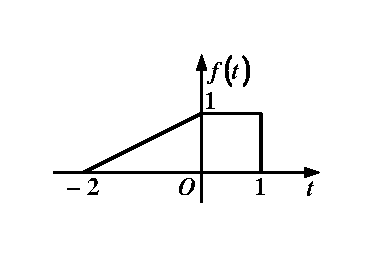
\includegraphics[width=40mm]{visio/1.7-a.pdf}
    \end{FigureSub}
    \begin{FigureSub}[反转信号$f(-t)$]
        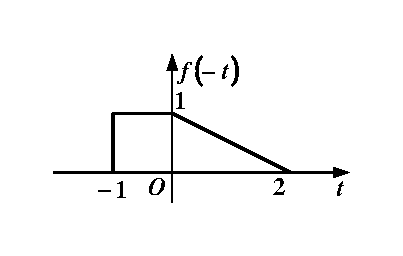
\includegraphics[width=40mm]{visio/1.7-b.pdf}
    \end{FigureSub}
\end{Figure}

\begin{BoxDefinition}[信号的反转]
    将$f(t)\rightarrow f(-t),f(k)\rightarrow f(-k)$称为对信号$f(\cdot)$的反转或反折。
\end{BoxDefinition}

\subsubsection{信号的平移}

\begin{Figure}[信号的平移]
    \begin{FigureSub}[平移前原始信号$f(t)$]
        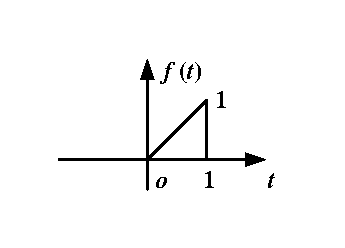
\includegraphics[width=40mm]{visio/1.8-a.pdf}
    \end{FigureSub}
    \begin{FigureSub}[平移信号$f(t-1)$]
        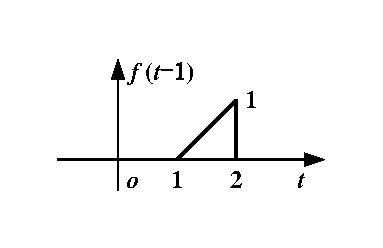
\includegraphics[width=40mm]{visio/1.8-b.pdf}
    \end{FigureSub}
\end{Figure}

\begin{BoxDefinition}[信号的平移]
    将$f(t)\rightarrow f(t-t_0),f(k)\rightarrow f(k-k_0)$称为对信号$f(\cdot)$的平移。

    若$t_0$(或$k_0$)$>0$,则将$f(\cdot)$右移,否则左移。
\end{BoxDefinition}

\subsubsection{信号的展缩}

\begin{Figure}[信号的展缩]
    \begin{FigureSub}[压缩前原始信号$f(t)$]
        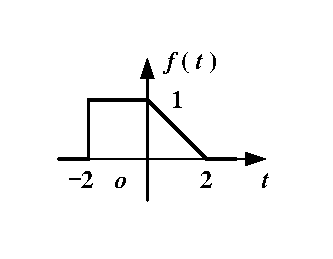
\includegraphics[width=40mm]{visio/1.9-a.pdf}
    \end{FigureSub}
    \begin{FigureSub}[压缩信号$f(2t)$]
        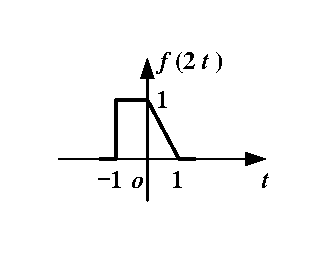
\includegraphics[width=40mm]{visio/1.9-b.pdf}
    \end{FigureSub}
\end{Figure}


\begin{BoxDefinition}[信号的展缩]
    将$f(t)\rightarrow f(at)$称为对信号$f(t)$的尺度变换。

    若$a>1$,则波形沿横坐标压缩。

    若$0<a<1$,则扩展。
\end{BoxDefinition}

离散信号一般不作尺度变换。

\subsubsection{信号的混合运算}

对正向运算$f(t)\rightarrow f(at+b)$,先平移再展缩最后再反转。

对逆向运算$f(at+b)\rightarrow f(t)$,先反转展缩,最后平移。

\subsection{信号的微分和积分}

\begin{Figure}[信号的微分]
    \begin{FigureSub}[微分前原始信号]
        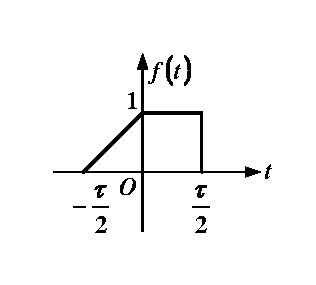
\includegraphics[width=40mm]{visio/1.10-a.pdf}
    \end{FigureSub}
    \begin{FigureSub}[信号微分]
        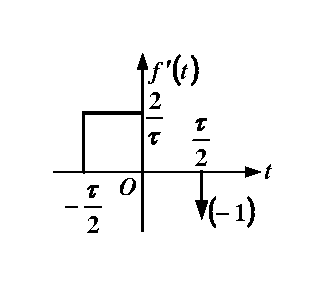
\includegraphics[width=40mm]{visio/1.10-b.pdf}
    \end{FigureSub}
\end{Figure}

\begin{Figure}[信号的积分]
    \begin{FigureSub}[积分前原始信号]
        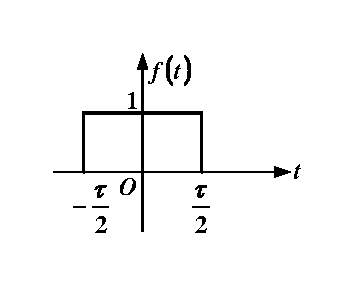
\includegraphics[width=40mm]{visio/1.11-a.pdf}
    \end{FigureSub}
    \begin{FigureSub}[信号积分]
        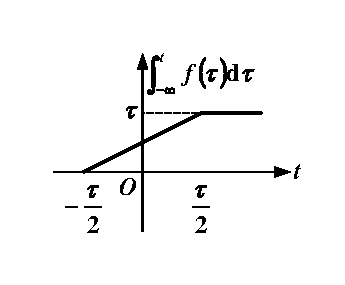
\includegraphics[width=40mm]{visio/1.11-b.pdf}
    \end{FigureSub}
\end{Figure}